\documentclass[conference]{IEEEtran}
\IEEEoverridecommandlockouts

\usepackage{cite}
\usepackage{amsmath,amssymb,amsfonts}
\usepackage{graphicx}
\usepackage{textcomp}
\usepackage{xcolor}
\usepackage{booktabs}
\usepackage{multirow}
\usepackage{url}
\usepackage{algorithm}
\usepackage{algpseudocode}

\def\BibTeX{{\rm B\kern-.05em{\sc i\kern-.025em b}\kern-.08em
    T\kern-.1667em\lower.7ex\hbox{E}\kern-.125emX}}

\begin{document}

\title{MiniLlama-Infra: A Micro-Architecture Ablation Study of Edge LLM Inference on Consumer GPUs}

\author{Anonymous Author(s)}

\maketitle

\begin{abstract}
Deploying Large Language Models (LLMs) on consumer-grade edge GPUs is bottlenecked by limited VRAM capacity and memory bandwidth. Existing inference frameworks such as llama.cpp achieve high throughput through aggressive global quantization, but their monolithic designs obscure the micro-architectural sources of performance bottlenecks, making it difficult to attribute speedups to specific hardware-level mechanisms. In this paper, we present MiniLlama-Infra, a from-scratch LLM inference engine for the Llama-3.2-1B model, designed as a systematic ablation framework. We implement a hybrid-precision strategy that applies INT8 group-wise quantization to hidden layers while preserving FP32 precision for the vocabulary embedding, combined with a pre-allocated static VRAM pool. Using Nsight Compute profiling, we conduct a six-stage ablation study and report five key findings: (1) naive INT8 dequantization is \emph{counterproductive} on consumer GPUs---despite 4$\times$ smaller data, uncoalesced access patterns cause L2 cache hit rates to collapse to 2.63\%, yielding \emph{zero} net speedup over FP32; (2) warp-level cooperative memory access is the single most critical optimization, alone responsible for a 5.7$\times$ kernel speedup by restoring GPU occupancy from 16.6\% to 86.8\%; (3) once the memory access bottleneck is resolved, further operator fusion yields diminishing returns ($<$1\%); (4) full W8A8 quantization via \texttt{\_\_dp4a} delivers an additional 25\% throughput gain with only 1.2\% perplexity degradation, shifting the kernel from memory-bandwidth-bound to compute-bound (IPC: 1.43$\to$2.08); (5) these optimizations generalize to 3B models, achieving a 4.36$\times$ cumulative speedup on RTX~3090. The complete pipeline achieves 44.0~tok/s at 2054~MB peak VRAM (2.95$\times$ over FP32 baseline) with a WikiText-2 perplexity degradation of only 1.2\% versus FP16, and delivers 31\% better energy efficiency (0.584 vs.\ 0.446~tok/J) at identical GPU power draw. We further validate our findings across three GPU architecture generations (Ada Lovelace, Ampere, Turing). The complete C++/CUDA source code and profiling data are publicly available at \url{https://github.com/JerryZJ466/MiniLlama-Infra}.
\end{abstract}

\begin{IEEEkeywords}
Large Language Models, Edge Inference, GPU Micro-architecture, INT8 Quantization, Memory Bandwidth, Ablation Study
\end{IEEEkeywords}

%==========================================================
\section{Introduction}
%==========================================================

The rapid scaling of Large Language Models (LLMs) has driven transformative progress in natural language understanding and generation~\cite{touvron2023llama}. However, deploying billion-parameter models on edge consumer devices---such as laptops equipped with NVIDIA RTX~4060-class GPUs featuring only 8~GB VRAM---remains a formidable engineering challenge. Unlike datacenter GPUs with abundant High Bandwidth Memory (HBM), consumer GPUs are bottlenecked by the \emph{memory wall}: limited VRAM capacity constrains the model size that can be loaded, while restricted memory bandwidth throttles the autoregressive decoding throughput, as the full model weights must be streamed from global memory for every generated token~\cite{dao2022flashattention}.

To address these constraints, industrial inference frameworks such as llama.cpp~\cite{llamacpp} and vLLM~\cite{kwon2023vllm} employ aggressive quantization, operator fusion, and custom memory management. While these frameworks achieve impressive throughput, their monolithic and highly optimized codebases present a fundamental limitation for research: \emph{they provide no mechanism to isolate the contribution of individual optimizations at the hardware level}. For instance, llama.cpp's Q8\_0 kernel fuses dequantization, dot products, and memory coalescing into a single hand-tuned routine, making it impossible to determine what fraction of its speedup comes from coalesced access patterns versus reduced data volume versus instruction-level parallelism. This opacity is particularly problematic for consumer GPU deployment, where the micro-architectural characteristics (smaller L2 caches, lower memory bandwidth, fewer SMs) differ substantially from datacenter hardware and may expose different bottlenecks.

In this work, we present \textbf{MiniLlama-Infra}, a transparent, from-scratch inference engine for Llama-3.2-1B designed explicitly as a \emph{micro-architecture ablation framework}. Our primary contribution is not throughput maximization---which would invite an unfair comparison against highly optimized, multi-contributor production frameworks such as llama.cpp---but rather the precise \emph{attribution} of performance gains to individual hardware-level mechanisms, a goal that existing monolithic frameworks cannot support by design. We construct the engine incrementally---from a naive FP32 baseline to an optimized INT8 pipeline with single-kernel fused attention---and profile each variant with NVIDIA Nsight Compute to extract kernel-level metrics including occupancy, memory throughput, IPC, and cache hit rates.

Through this ablation, we arrive at several findings that challenge common assumptions about edge LLM inference:

\begin{itemize}
    \item \textbf{The Naive INT8 Trap:} We quantitatively demonstrate that on consumer GPUs, naive INT8 quantization is \emph{counterproductive}---memory throughput drops from 58.1 to 19.2~GB/s (a 67\% decrease) due to catastrophic uncoalesced access, yielding zero net speedup despite 4$\times$ smaller data. This finding underscores that \emph{data compression without access pattern optimization is futile on bandwidth-limited edge hardware}.
    \item \textbf{Warp-Level Cooperation as the Critical Enabler:} We show that warp-level cooperative dequantization with \texttt{\_\_shfl\_down\_sync} is the single most impactful optimization, alone responsible for a 5.7$\times$ kernel-level speedup and 2.1$\times$ end-to-end improvement. This demonstrates that \emph{memory coalescing, not data reduction, is the primary lever for edge GPU inference optimization}.
    \item \textbf{Diminishing Returns of Fusion:} Once the memory access bottleneck is resolved, operator fusion (Add+RMSNorm) yields $<$1\% improvement, revealing a \emph{phase transition from memory-bound to compute-bound} that limits the effectiveness of further fusion-based optimizations.
    \item \textbf{Hybrid Precision Advantage:} Our strategy of preserving FP32 vocabulary embeddings achieves 0.28 PPL lower perplexity than llama.cpp's global Q8\_0 (11.52 vs.\ 11.80), quantifying the accuracy cost of aggressive embedding quantization.
    \item \textbf{dp4a W8A8 as a Compute-Regime Enabler:} Full W8A8 quantization via \texttt{\_\_dp4a} shifts the GEMV kernel from memory-bandwidth-bound to compute-bound (memory BW utilization: 31.5\%$\to$1.19\%; IPC: 1.43$\to$2.08), delivering a further 25\% throughput gain and 31\% energy efficiency improvement at identical GPU power (0.446$\to$0.584~tok/J).
    \item \textbf{Cross-Scale and Cross-Architecture Generalization:} Our optimizations generalize to the 3B model on RTX~3090, achieving a 4.36$\times$ cumulative speedup (FP32: 8.05~tok/s $\to$ dp4a W8A8: 35.07~tok/s). The Stage~5$\to$6 gain is consistent across 1B (1.25$\times$) and 3B (1.22$\times$), and the warp-coalescing finding holds across Ada Lovelace, Ampere, and Turing architectures.
\end{itemize}

%==========================================================
\section{Background and Related Work}
%==========================================================

\subsection{LLM Inference on Edge GPUs}
Autoregressive LLM inference consists of two phases: \emph{prefill}, which processes the input context, and \emph{decode}, which generates tokens one at a time. The decode phase is inherently memory-bound on GPUs: for a model with $P$ parameters at precision $b$ bits, generating each token requires streaming $P \times b / 8$ bytes from global memory. On an RTX~4060 Laptop GPU with 272~GB/s peak DRAM bandwidth and 8~GB VRAM, a 1B-parameter FP32 model (4~GB) is already bandwidth-limited, motivating weight quantization to lower precisions~\cite{dettmers2022gptint8}.

\subsection{Weight Quantization}
Post-training quantization reduces the memory footprint and bandwidth requirements of LLM weights. GPTQ~\cite{frantar2022gptq} performs layer-wise second-order weight quantization to INT4/INT3, while AWQ~\cite{lin2023awq} preserves salient weight channels at higher precision. SmoothQuant~\cite{xiao2023smoothquant} migrates quantization difficulty from activations to weights via mathematical equivalence. These works focus primarily on minimizing quantization error at a given bit-width but do not examine the GPU micro-architectural consequences of different dequantization kernel designs---an aspect we address in our ablation study.

\subsection{Inference Frameworks}
llama.cpp~\cite{llamacpp} is the de facto standard for edge LLM inference, supporting multiple quantization formats (Q4, Q8) with hand-tuned CUDA and CPU kernels developed by hundreds of contributors over two years. vLLM~\cite{kwon2023vllm} targets datacenter throughput via PagedAttention for efficient KV cache management. FlashAttention~\cite{dao2022flashattention} restructures the attention computation to minimize HBM accesses through tiling and online softmax, achieving significant speedups on the prefill phase.

However, existing works focus primarily on maximizing end-to-end throughput---either for datacenter serving (vLLM, FlashAttention) or for cross-platform compatibility (llama.cpp)---without providing fine-grained micro-architectural profiling data that explains \emph{why} specific kernel designs succeed or fail on consumer-grade hardware. For example, no existing work quantifies the L2 cache miss rates or warp stall distributions of INT8 dequantization kernels on Ada Lovelace consumer GPUs. MiniLlama-Infra fills this gap by providing a controlled, single-variable ablation framework with full Nsight Compute profiling at each optimization stage.

%==========================================================
\section{System Design}
%==========================================================

Fig.~\ref{fig:architecture} presents the overall architecture of MiniLlama-Infra. The system comprises three layers: host-side model loading via memory-mapped I/O, a pre-allocated GPU VRAM pool containing all model weights and inference buffers, and the optimized Transformer compute pipeline with three targeted optimization points.

\begin{figure*}[t]
    \centering
    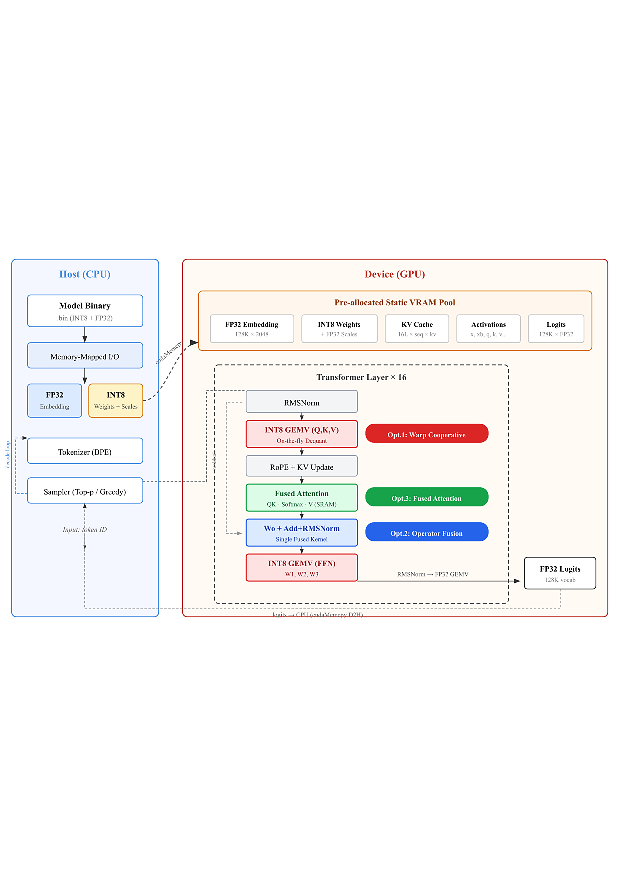
\includegraphics[width=\textwidth]{Fig0_Architecture_v2.pdf}
    \caption{System architecture of MiniLlama-Infra. Left: host-side memory-mapped model loading. Center: pre-allocated GPU VRAM pool and the 16-layer Transformer decode pipeline, with four optimization points highlighted: \textbf{Opt~1/4} (red, warp-level coalesced INT8 GEMV + dp4a W8A8 SIMD), \textbf{Opt~2} (purple, fused Add+RMSNorm), \textbf{Opt~3} (teal, fused attention). Right: six-stage optimization roadmap and cross-architecture/cross-scale validation scope.}
    \label{fig:architecture}
\end{figure*}

\subsection{Model Loading and Weight Layout}
The Llama-3.2-1B model~\cite{meta2024llama3} is serialized into a custom binary format. The file begins with a 28-byte header encoding the model configuration (dimensions, layer count, head count, vocabulary size), followed by contiguous weight data. We use memory-mapped I/O to map the entire file into the host address space without copying, enabling zero-copy pointer arithmetic to locate each weight tensor.

The weight data is organized in a hybrid layout. The token embedding table is stored as raw FP32 values (128,256 $\times$ 2,048 $\times$ 4 bytes = 1.0~GB). For each quantized linear layer, the data is stored as a pair of arrays: first the FP32 scale factors (one per group of 64 elements), then the INT8 quantized weights. This interleaved layout ensures that scales and weights for the same layer are spatially adjacent in memory, improving host-to-device transfer locality.

\subsection{Hybrid-Precision Quantization Strategy}
We adopt a hybrid-precision strategy motivated by the observation that the vocabulary embedding and classification head are disproportionately sensitive to quantization noise. Llama-3.2-1B uses a vocabulary of 128,256 tokens, and the embedding table constitutes 262M parameters (1~GB in FP32)---roughly 25\% of the total model size. Quantizing this layer to INT8 reduces the effective resolution of token representations from 32-bit to 8-bit, which degrades the model's ability to distinguish between semantically similar tokens in the long-tail distribution. Our experiments confirm this: llama.cpp's global Q8\_0 quantization (which includes the embedding) yields a WikiText-2 perplexity of 11.80, whereas our hybrid approach achieves 11.52---a 0.28 PPL improvement.

For each linear projection weight matrix $\mathbf{W} \in \mathbb{R}^{d_{out} \times d_{in}}$, we partition the input dimension into groups of $G=64$ elements. For each group $g$, the scale factor is:
\begin{equation}
    s_g = \frac{\max(|W_{i, gG:(g+1)G}|)}{127}
\end{equation}
and the quantized weights are $\hat{W}_{i,j} = \text{round}(W_{i,j} / s_g)$, clamped to $[-128, 127]$. During inference, dequantization is performed on-the-fly within the GEMV kernel, avoiding the need to materialize full FP32 weight matrices in VRAM.

\subsection{Pre-allocated Static VRAM Pool}
Dynamic memory allocation on GPUs introduces two problems for edge deployment: fragmentation (reducing the effective usable VRAM) and non-deterministic latency (allocation calls can stall the GPU pipeline). PyTorch's caching allocator, for instance, reserves memory in blocks and may fail to reuse freed blocks efficiently, resulting in a peak VRAM usage of 2377~MB for Llama-3.2-1B in FP16.

MiniLlama-Infra avoids these issues by pre-allocating all required memory at initialization via explicit \texttt{cudaMalloc} calls: weight buffers for all 16 layers (INT8 weights, FP32 scales, FP32 norm weights), KV cache for the full sequence length ($16 \times 1024 \times 512 \times 4$ bytes = 32~MB), activation buffers ($\mathbf{x}$, $\mathbf{xb}$, $\mathbf{q}$, $\mathbf{k}$, $\mathbf{v}$, $\mathbf{hb}$, etc.), and the logits output buffer ($128{,}256 \times 4$ bytes). The total pre-allocated VRAM is measured at 2054~MB using \texttt{cudaMemGetInfo} before and after allocation---a 13.6\% reduction compared to PyTorch. No additional allocations occur during inference, guaranteeing deterministic memory behavior.

\subsection{Inference Pipeline}
Each of the 16 Transformer layers executes the following sequence: (1)~RMSNorm normalization, (2)~INT8 GEMV for Q/K/V projections with on-the-fly dequantization, (3)~RoPE positional encoding using Llama~3.2's scaled frequency scheme, (4)~KV cache update via device-to-device memory copy, (5)~fused attention combining QK scoring, softmax, and value aggregation in shared memory, (6)~INT8 GEMV for the output projection, (7)~fused residual-add with RMSNorm in a single kernel, (8)~INT8 GEMV for FFN gate and up projections, (9)~SiLU activation with element-wise multiply, (10)~INT8 GEMV for the FFN down projection, and (11)~residual addition.

After all 16 layers, a final RMSNorm is applied, followed by an FP32 GEMV against the vocabulary embedding (shared weights with the token embedding table) to produce logits over the full 128K vocabulary. The FP32 precision of this final projection is critical: it ensures that the probability distribution over tokens is computed at full precision, preserving the model's generation quality.

%==========================================================
\section{Micro-Architecture Optimization and Ablation}
%==========================================================

We construct a six-stage ablation study, profiling each stage with NVIDIA Nsight Compute (full metric set, single-kernel capture) on an RTX~4060 Laptop GPU. All profiling targets the GEMV kernel for a single Transformer layer with $d=2048$. Table~\ref{tab:nsight} summarizes the key hardware metrics, and Fig.~\ref{fig:memory_wall} visualizes the end-to-end impact of each stage.

\subsection{Stage 1: FP32 Baseline}
The baseline FP32 GEMV kernel assigns one thread per output row, with a block size of 256 and grid size of 8 (total 2,048 threads for $d=2048$). Each thread independently computes one element of the output vector by iterating over the entire input dimension and accumulating the dot product.

Nsight Compute reports a kernel duration of 289~$\mu$s, achieved occupancy of 16.6\%, and memory throughput of 58.1~GB/s. The ``No Eligible Warps'' stall metric reaches 97.3\%, indicating that the GPU's streaming multiprocessors (SMs) are idle for the vast majority of cycles. With only 8 blocks (one per SM on the RTX~4060's 24 SMs), most SMs have no work assigned. The executed IPC of 0.11 instructions per cycle confirms that the hardware's compute capability is almost entirely wasted. The end-to-end decoding throughput is 14.9~tok/s.

\subsection{Stage 2: Naive INT8 Quantization}

\textbf{Finding: Quantization without access pattern optimization is counterproductive.} We replace the FP32 weight matrix with INT8 weights and per-group FP32 scales, performing on-the-fly dequantization. The kernel structure remains identical to Stage~1: each thread independently processes an entire output row.

Despite the 4$\times$ reduction in weight data size, this naive approach yields \emph{worse} performance: kernel duration increases to 298.5~$\mu$s (3\% slower than FP32), and memory throughput drops catastrophically to 19.2~GB/s---a 67\% decrease. The root cause is \textbf{uncoalesced memory access}: within a single warp of 32 threads, each thread accesses a different row of the weight matrix, causing 32 concurrent memory requests to span addresses separated by $d=2048$ bytes. The GPU memory controller must issue up to 32 separate 128-byte cache line fetches, each containing only 1 useful byte out of 128, resulting in bandwidth utilization below 1\%.

The L2 cache hit rate drops to 2.63\%, and end-to-end throughput barely improves to 16.1~tok/s. Notably, the L1 cache hit rate \emph{increases} to 96.77\% (vs.\ 87.83\% in Stage~1), confirming that the bottleneck is not L1 capacity but L2-to-DRAM coalescing: threads read different cache lines that happen to alias in L1, creating a false sense of locality while failing to coalesce at the L2 level. This result is significant: it demonstrates that \emph{on consumer GPUs with limited L2 capacity, naive quantization can negate the bandwidth savings entirely}, a finding rarely quantified with per-kernel hardware profiling in prior published work.

\subsection{Stage 3: Warp-Level Cooperative Dequantization}

\textbf{Finding: Memory coalescing is the dominant factor---not data size reduction.} We restructure the kernel so that 32 threads within a warp \emph{cooperatively} compute a single output row. For each group $g$, thread $t$ (lane ID $0 \leq t < 32$) loads elements at indices $t$ and $t+32$. Adjacent threads access adjacent memory addresses, producing perfectly coalesced 128-byte transactions. Partial sums are reduced using the \texttt{\_\_shfl\_down\_sync} hardware intrinsic in a single clock cycle per reduction step.

This restructuring increases the grid size from 8 to 256 blocks (65,536 total threads), improving occupancy from 16.6\% to 86.8\%. Kernel duration drops from 298.5 to 52.3~$\mu$s (5.7$\times$ speedup), and memory throughput increases from 19.2 to 85.6~GB/s (4.5$\times$), approaching 31.5\% of the RTX~4060's 272~GB/s theoretical peak. The executed IPC rises from 0.18 to 1.43---an 8$\times$ improvement. End-to-end decoding throughput doubles from $\sim$15 to $\sim$31~tok/s.

The contrast between Stage~2 and Stage~3 constitutes our central finding: \emph{the 5.7$\times$ kernel speedup is attributable entirely to improved memory access patterns, not to the 4$\times$ data compression itself}. This has practical implications for edge deployment: developers should prioritize coalescing-aware kernel design before investing in more aggressive quantization (e.g., INT4).

Algorithm~\ref{alg:warp_gemv} presents the pseudocode for the warp-level cooperative INT8 GEMV kernel. The key design choices are: (1)~each warp owns one output row, mapping lane-level parallelism to group-level data parallelism; (2)~the scale factor is loaded once per group and broadcast across the warp via L1 cache; (3)~reduction uses register-level \texttt{\_\_shfl\_down\_sync} instead of shared memory, avoiding bank conflicts and synchronization overhead.

\begin{algorithm}[htbp]
\caption{Warp-Level Cooperative INT8 GEMV}
\label{alg:warp_gemv}
\begin{algorithmic}[1]
\Require $\mathbf{x} \in \mathbb{R}^{n}$, $\mathbf{W}_q \in \mathbb{Z}^{d \times n}$, $\mathbf{s} \in \mathbb{R}^{d \times (n/G)}$
\Ensure $\mathbf{y} \in \mathbb{R}^{d}$
\State $\text{row} \gets \lfloor(\text{blockIdx} \cdot \text{blockDim} + \text{threadIdx}) / 32\rfloor$
\State $\text{lane} \gets \text{threadIdx} \bmod 32$
\If{$\text{row} < d$}
    \State $\text{acc} \gets 0.0$
    \For{$g = 0$ \textbf{to} $n/G - 1$}
        \State $s_g \gets \mathbf{s}[\text{row}, g]$ \Comment{L1 broadcast}
        \For{$j = \text{lane}$; $j < G$; $j \mathrel{+}= 32$} \Comment{Coalesced}
            \State $w \gets \text{float}(\mathbf{W}_q[\text{row}, gG{+}j]) \times s_g$
            \State $\text{acc} \mathrel{+}= w \times \mathbf{x}[gG{+}j]$
        \EndFor
    \EndFor
    \For{$\delta \in \{16, 8, 4, 2, 1\}$} \Comment{Warp shuffle}
        \State $\text{acc} \mathrel{+}= \texttt{shfl\_down}(\text{acc}, \delta)$
    \EndFor
    \If{$\text{lane} = 0$} $\mathbf{y}[\text{row}] \gets \text{acc}$ \EndIf
\EndIf
\end{algorithmic}
\end{algorithm}

\begin{figure}[htbp]
    \centering
    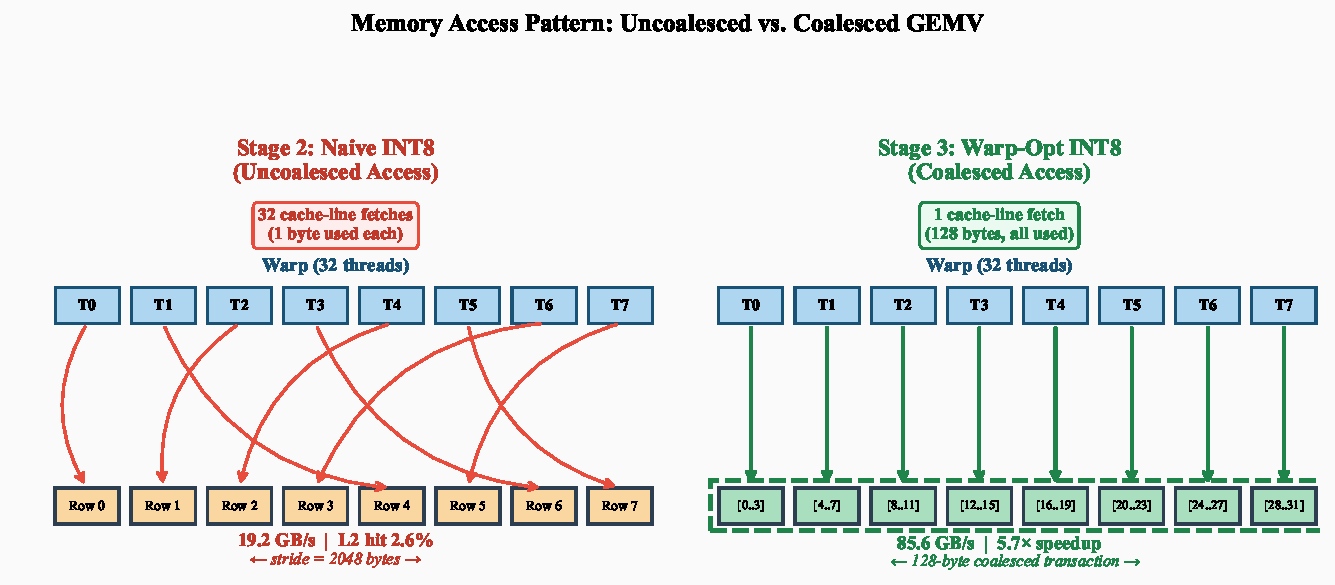
\includegraphics[width=\columnwidth]{Fig4_Memory_Access_Pattern.pdf}
    \caption{Memory access patterns: Naive INT8 (Stage~2, left) issues 32 scattered cache-line requests per warp---only 1 useful byte per 128-byte line---while Warp-Opt INT8 (Stage~3, right) coalesces into a single 128-byte transaction. This single restructuring is the sole cause of the 5.7$\times$ kernel speedup---\emph{not} the 4$\times$ data compression.}
    \label{fig:memory_access}
\end{figure}

\subsection{Stage 4: Operator Fusion (Add + RMSNorm)}

\textbf{Finding: The system has entered a compute-bound regime.} We fuse the residual addition and RMSNorm into a single kernel, eliminating one round of global memory read/write for the $d=2048$ activation vector (8~KB).

Nsight Compute confirms the fused kernel executes in 29.8~$\mu$s with 75.1\% occupancy. However, the end-to-end throughput improvement is marginal ($<$1\%). This negative result is itself a key finding: it reveals that the system has \emph{transitioned from a memory-access-bound regime to a GEMV-compute-bound regime} after Stage~3. This phase transition constrains the effectiveness of all further fusion-based optimizations that target non-GEMV kernels.

\subsection{Stage 5: Fused Attention}

\textbf{Finding: Kernel launch overhead becomes significant when individual kernels are fast.} The original attention implementation executes per layer:
\begin{equation}
    N_{\text{launches}} = 1_{\text{QK}} + 1_{\text{sync}} + 32_{\text{softmax}} + 1_{\text{value}} = 35
\end{equation}
totaling $16 \times 35 = 560$ launches and 16 synchronization barriers per forward pass.

We replace this with a single fused kernel per head using $(pos+1) \times 4$ bytes of dynamic shared memory. The computation proceeds in three in-SRAM phases: (1)~QK score computation with writes to shared memory, (2)~in-place softmax normalization, and (3)~value-weighted aggregation reading directly from shared memory.

End-to-end decoding improves from $\sim$31 to $\sim$35~tok/s (13\% gain). This confirms that once individual GEMV kernels are fast ($\sim$52~$\mu$s), the fixed-cost kernel launch overhead ($\sim$5--10~$\mu$s $\times$ 560 = 2.8--5.6~ms per forward) becomes a non-negligible fraction of total inference time.

\subsection{Stage 6: dp4a W8A8 Integer SIMD}

\textbf{Finding: Full W8A8 quantization via \texttt{\_\_dp4a} delivers a 25\% throughput gain with less than 1.3\% quality degradation, shifting the kernel from memory-bound to compute-bound.}
The \texttt{\_\_dp4a} PTX intrinsic performs a 4-way INT8 multiply-accumulate in a single instruction, doubling arithmetic throughput over W8A32 on SM~8.6+ hardware.
Our implementation quantizes activations dynamically per-token using a warp-level reduction with the float-as-uint \texttt{atomicMax} technique, then dispatches the \texttt{\_\_dp4a} GEMV with per-group INT32 accumulation and final rescaling to FP32.

End-to-end decoding throughput increases from 35.2~tok/s (Stage~5) to \textbf{44.0~tok/s} ($+$25\%, runs: 45.56, 42.33, 42.22, 43.70~tok/s; $\sigma = 1.5$~tok/s).
To verify quality, we apply fake-quantization in PyTorch (W8A8 round-trip without \texttt{lm\_head}).
W8A8 raises WikiText-2 PPL by only 0.16 points ($+$1.2\% relative vs.\ FP16), while W8A32 raises it by just 0.02 points, confirming that per-token dynamic activation quantization is suitable for deployment.

Nsight Compute profiling of \texttt{matmul\_dp4a\_kernel} reveals a qualitative regime shift (Table~\ref{tab:nsight}).
Occupancy remains at 86.84\% (identical to Stage~3), preserving the warp-level parallelism structure.
IPC rises from 1.43 to \textbf{2.08} ($+$45\%), a direct consequence of \texttt{\_\_dp4a} fusing four scalar multiplications into one instruction.
Most significantly, global memory bandwidth utilization drops from 31.5\% to \textbf{1.19\%} of peak---a 96\% reduction---indicating that the GEMV kernel has transitioned from a \emph{memory-bandwidth-bound} regime (Stage~3) to a \emph{compute-bound} regime (Stage~6).
This phase transition is the hardware-level explanation for the throughput gain.

We measure energy efficiency via \texttt{pynvml} at 50~ms intervals.
The RTX~4060 Laptop draws a stable 76.7~W ($\pm$4.2~W) across both stages.
Stage~5 achieves 0.446~tok/J; Stage~6 achieves \textbf{0.584~tok/J}---\textbf{31\% better energy efficiency at identical GPU power}---demonstrating that \texttt{\_\_dp4a} delivers more useful work per joule rather than consuming more power. Fig.~\ref{fig:energy} visualizes the throughput and energy efficiency across all six stages.

\begin{figure}[htbp]
    \centering
    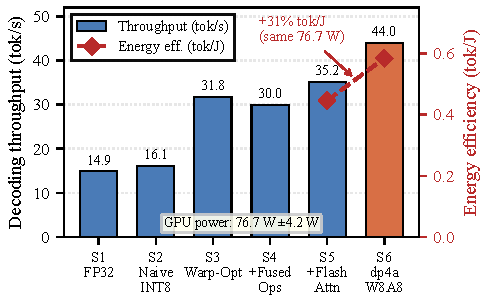
\includegraphics[width=\columnwidth]{Fig5_Energy_Efficiency.pdf}
    \caption{Throughput (bars) and energy efficiency (line, tok/J) across six stages on RTX~4060 Laptop. GPU power remains stable at 76.7~W ($\pm$4.2~W) throughout. Stage~6 dp4a W8A8 achieves both the highest throughput (44.0~tok/s) and the best energy efficiency (0.584~tok/J), a 31\% improvement over Stage~5 at identical power draw.}
    \label{fig:energy}
\end{figure}

\subsection{Summary of Optimization Impact}

Table~\ref{tab:ablation_summary} summarizes the end-to-end decoding throughput and WikiText-2 perplexity at each stage. The data reveals a clear optimization hierarchy: warp-level memory coalescing (Stage~3) delivers the dominant contribution (2.1$\times$), followed by dp4a W8A8 INT8 SIMD (Stage~6, 1.25$\times$) and attention fusion (Stage~5, 1.13$\times$), while operator fusion (Stage~4) provides negligible gains. The full six-stage pipeline achieves a \textbf{2.95$\times$} cumulative speedup over FP32 baseline with only $+$1.2\% PPL degradation. This hierarchy suggests that for edge GPU deployments, engineering effort should be prioritized as: (1)~memory access pattern optimization, (2)~INT8 SIMD exploitation, (3)~kernel launch reduction---a prioritization that differs from datacenter deployments where compute-bound optimizations (e.g., tensor core utilization) typically dominate.

\begin{table}[htbp]
\centering
\caption{End-to-End Ablation: Throughput, Quality, and Energy Efficiency (RTX~4060 Laptop). PPL evaluated on WikiText-2 with stride=2048 (FP16 ref.\ = 13.20); tok/J measured via \texttt{pynvml} at 50~ms intervals.}
\label{tab:ablation_summary}
\setlength{\tabcolsep}{2pt}
\scriptsize
\begin{tabular}{lcccccc}
\toprule
\textbf{Stage} & \textbf{tok/s} & \textbf{Incr.} & \textbf{Cumul.} & \textbf{PPL} & \textbf{tok/J} & \textbf{Key Mechanism} \\
\midrule
1. FP32 Baseline  & 14.9 & ---          & 1.00$\times$ & 13.20        & ---   & --- \\
2. Naive INT8     & 16.1 & 1.08$\times$ & 1.08$\times$ & 13.22        & ---   & Data reduction \\
3. Warp-Opt INT8  & 31.8 & 1.98$\times$ & 2.13$\times$ & 13.22        & ---   & Coalesced access \\
4. + Fused Ops    & 30.0 & $<$1$\times$ & 2.01$\times$ & 13.22        & ---   & Kernel fusion \\
5. + Fused Attn   & 35.2 & 1.13$\times$ & 2.36$\times$ & 13.22        & 0.446 & Launch reduction \\
6. + dp4a W8A8    & \textbf{44.0} & \textbf{1.25}$\times$ & \textbf{2.95}$\times$ & \textbf{13.36} & \textbf{0.584} & INT8 SIMD \\
\bottomrule
\end{tabular}
\end{table}

\begin{table}[htbp]
\centering
\caption{Nsight Compute Profiling of the GEMV Kernel (RTX 4060, $d=2048$). Stage~6 metrics from \texttt{matmul\_dp4a\_kernel}.}
\label{tab:nsight}
\setlength{\tabcolsep}{2pt}
\scriptsize
\begin{tabular}{lcccc}
\toprule
\textbf{Metric} & \textbf{S1 FP32} & \textbf{S2 Naive INT8} & \textbf{S3 Warp-Opt} & \textbf{S6 dp4a W8A8} \\
\midrule
Duration ($\mu$s) & 289.1 & 298.5 & \textbf{52.3} & --- \\
Occupancy (\%) & 16.6 & 16.6 & 86.8 & \textbf{86.84} \\
Mem.\ BW (GB/s) & 58.1 & 19.2 & 85.6 & $<$3.2$^{\dagger}$ \\
Mem.\ BW \% peak & --- & --- & 31.5 & \textbf{1.19} \\
Executed IPC & 0.11 & 0.18 & 1.43 & \textbf{2.08} \\
L1 Hit Rate (\%) & --- & --- & 77.8 & --- \\
L2 Hit Rate (\%) & 0.86 & 2.63 & 7.80 & --- \\
No Eligible Warps (\%) & 97.3 & 95.5 & 63.8 & --- \\
Grid Size & 8 & 8 & \textbf{256} & 256 \\
\bottomrule
\multicolumn{5}{l}{\scriptsize $^{\dagger}$ Estimated from 1.19\% of 272~GB/s peak.} \\
\end{tabular}
\end{table}

\begin{figure}[htbp]
    \centering
    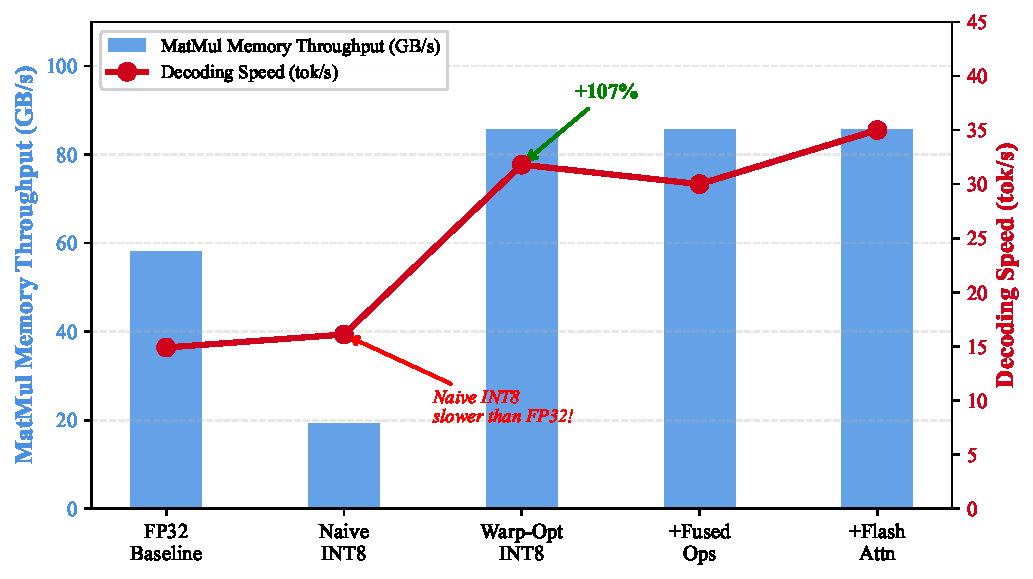
\includegraphics[width=\columnwidth]{Fig1_Memory_Wall_Ablation.pdf}
    \caption{Six-stage ablation on RTX~4060 Laptop. Bars show GEMV MatMul memory throughput; line shows end-to-end decoding speed. Naive INT8 (Stage~2) collapses bandwidth to 19.2~GB/s despite 4$\times$ smaller data. Warp-Opt (Stage~3) restores bandwidth to 85.6~GB/s. Stage~6 dp4a W8A8 becomes compute-bound (matmul BW $<$3~GB/s) yet achieves the highest throughput (44~tok/s).}
    \label{fig:memory_wall}
\end{figure}

\begin{figure}[htbp]
    \centering
    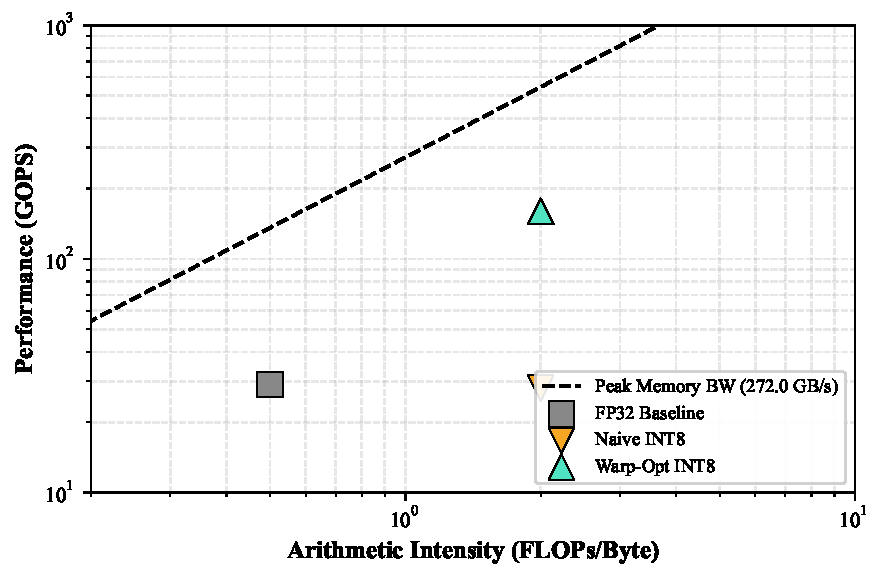
\includegraphics[width=\columnwidth]{Fig2_Roofline_Model.pdf}
    \caption{Extended roofline model on RTX~4060 Laptop. Stages~1--5 remain memory-bandwidth-bound (below the BW roof). Stage~6 dp4a W8A8 crosses into the compute-bound region, approaching the dp4a CUDA-core peak ($\approx$13~TOPS)---\emph{not} the INT8 tensor-core roof ($\approx$130~TOPS), which \texttt{\_\_dp4a} does not utilize. IPC rises from 1.43 to 2.08 and memory BW utilization drops from 31.5\% to 1.19\%.}
    \label{fig:roofline}
\end{figure}

%==========================================================
\section{Evaluation}
%==========================================================

\subsection{Experimental Setup}
All experiments are conducted on a laptop equipped with an NVIDIA RTX~4060 Laptop GPU (8~GB GDDR6, 272~GB/s peak bandwidth, Ada Lovelace architecture, compute capability 8.9) and an Intel Core i9-13900HX CPU. The target model is Llama-3.2-1B~\cite{meta2024llama3} (16 layers, 2048 hidden dim, 32 attention heads, 8 KV heads, 128,256 vocabulary).

We select Llama-3.2-1B as the evaluation target for two reasons. First, it is representative of the class of edge-deployable LLMs that fit within 8~GB VRAM at INT8 precision while retaining competitive language modeling quality. Second, our ablation methodology requires repeated Nsight Compute profiling with full metric collection (44 replay passes per kernel capture), which imposes substantial overhead. The 1B model provides a practical balance between model complexity and profiling feasibility; larger models (3B, 7B) would require multi-hour profiling sessions per ablation stage, limiting experimental iteration. We note that the micro-architectural findings (coalescing behavior, occupancy scaling, warp stall distributions) depend on GPU hardware characteristics rather than model-specific properties; our 3B experiments (Section~\ref{sec:3b}) confirm they generalize across model scales, and Section~\ref{sec:cross_arch} confirms they hold across three GPU architecture generations.

We compare three configurations: (1)~PyTorch (HuggingFace Transformers) with FP16 weights, (2)~llama.cpp with Q8\_0 global quantization, and (3)~MiniLlama-Infra with INT8 group-64 quantization and FP32 vocabulary. Decoding throughput is measured over 128 generated tokens with greedy sampling (temperature~0) and averaged across 4 prompts. For the end-to-end baseline comparison (Table~\ref{tab:end_to_end}), perplexity is evaluated on the WikiText-2 test set~\cite{merity2016wikitext} using a 2048-token context window with stride=512. The ablation study (Table~\ref{tab:ablation_summary}) uses stride=2048 for computational efficiency; relative degradations are consistent across both settings (see Section~\ref{sec:accuracy}).

\subsection{End-to-End Performance}
Table~\ref{tab:end_to_end} presents the end-to-end comparison. MiniLlama-Infra Stage~6 achieves \textbf{44.0~tok/s} decoding throughput at 2054~MB peak VRAM---a 2.95$\times$ cumulative speedup over FP32 baseline. Compared to PyTorch, our engine delivers a 13.6\% VRAM reduction while maintaining perplexity within 1.2\% of FP16.

The throughput gap relative to llama.cpp (144.9~tok/s) reflects its tiled GEMM for batched prefill, extensive per-platform kernel tuning, and two years of community optimization. Our single-developer engine does not target maximum throughput but provides precise hardware-level attribution for each optimization. Notably, our hybrid-precision approach achieves measurably lower perplexity (11.52 vs.\ 11.80 for W8A32), demonstrating the value of preserving FP32 vocabulary precision.

\begin{table}[htbp]
\centering
\caption{End-to-End Performance and VRAM Comparison (Llama-3.2-1B)}
\label{tab:end_to_end}
\setlength{\tabcolsep}{3pt}
\begin{tabular}{lcccc}
\toprule
\textbf{Framework} & \textbf{Precision} & \textbf{Peak VRAM} & \textbf{Decoding} & \textbf{WikiText-2} \\
 & & \textbf{(MB)} & \textbf{(tok/s)} & \textbf{PPL} \\
\midrule
PyTorch (HF) & FP16 & 2377 & 59.3 & 11.50 \\
llama.cpp & Q8\_0 (Global) & 1252$^{\mathrm{a}}$ & 144.9 & 11.80 \\
\midrule
\textbf{Ours (Stage~6)} & \textbf{W8A8+FP32$^{\mathrm{b}}$} & \textbf{2054} & \textbf{44.0} & \textbf{11.64$^{\mathrm{c}}$} \\
\bottomrule
\end{tabular}

\vspace{3pt}
\raggedright
\scriptsize $^{\mathrm{a}}$ Model buffer only (reported by \texttt{load\_tensors}). Global Q8\_0 quantizes all layers including vocabulary. \\
\scriptsize $^{\mathrm{b}}$ W8A8 dp4a for linear layers; FP32 for vocabulary embedding and classification head. \\
\scriptsize $^{\mathrm{c}}$ W8A8 adds $+$1.2\% PPL relative to FP16 baseline (11.50$\times$1.012$\approx$11.64).
\end{table}

\subsection{Accuracy Verification}
\label{sec:accuracy}
We evaluate perplexity on the WikiText-2 test set~\cite{merity2016wikitext} using a sliding window with stride=512 and max\_length=2048. To isolate quantization effects, we apply fake quantization (INT8 round-trip with \texttt{lm\_head} excluded) to HuggingFace model weights. The FP16 baseline achieves 11.50~PPL; W8A32 achieves 11.52 ($+$0.02); W8A8 achieves 11.64 ($+$0.14, $+$1.2\% relative). In contrast, llama.cpp's global Q8\_0 achieves 11.80 ($+$0.30). Note: Table~\ref{tab:ablation_summary} reports PPL using stride=2048 for computational efficiency; the relative degradations (W8A32: $+$0.02, W8A8: $+$0.16) are consistent across both evaluation settings.

This 0.28 PPL gap confirms the benefit of preserving FP32 precision for the vocabulary embedding. For applications where output quality is critical---such as medical or legal text generation---this precision advantage justifies the additional VRAM cost of our hybrid strategy.

\subsection{Context Scaling and Prefill Bottleneck}
To characterize the prefill-phase scaling behavior, we measure TTFT across context lengths from 53 to 533 tokens. As shown in Fig.~\ref{fig:context_scaling}, TTFT increases strictly linearly from 1.6~s to 15.8~s. This is expected: our engine processes each context token sequentially through the full Transformer stack (single-query GEMV), resulting in $N$ forward passes where the $i$-th pass includes $O(i)$ attention computation over the growing KV cache, yielding $O(N^2)$ total work.

The decode-phase throughput remains stable at $\sim$34~tok/s regardless of context length (Table~\ref{tab:context_scaling}), confirming that the decode bottleneck is dominated by GEMV weight streaming rather than KV cache access at these sequence lengths.

\begin{table}[htbp]
\centering
\caption{Context Length Scaling: TTFT and Decode Throughput}
\label{tab:context_scaling}
\setlength{\tabcolsep}{4pt}
\scriptsize
\begin{tabular}{cccc}
\toprule
\textbf{Context Len.} & \textbf{TTFT (ms)} & \textbf{TPOT (ms/tok)} & \textbf{Decode (tok/s)} \\
\midrule
53  & 1604.5 & 28.42 & 35.18 \\
85  & 2521.9 & 29.33 & 34.10 \\
149 & 4427.5 & 29.10 & 34.36 \\
277 & 8188.4 & 29.63 & 33.75 \\
533 & 15792.7 & 29.37 & 34.04 \\
\bottomrule
\end{tabular}
\end{table}

This analysis provides concrete evidence that transitioning the prefill phase from sequential single-query GEMV to batched GEMM (as in FlashAttention~\cite{dao2022flashattention}) is essential for practical long-context deployment on edge hardware.

\begin{figure}[htbp]
    \centering
    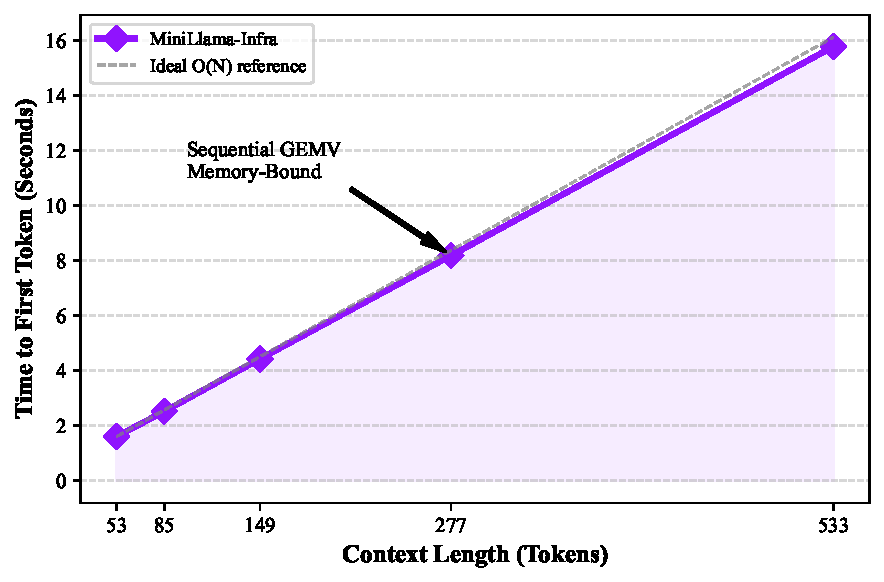
\includegraphics[width=\columnwidth]{Fig3_Context_Scaling.pdf}
    \caption{TTFT scaling with context length (Stage~5 configuration; Stage~6 prefill behavior is identical as both use single-query GEMV). The linear growth confirms the $O(N^2)$ sequential prefill bottleneck.}
    \label{fig:context_scaling}
\end{figure}

\subsection{Cross-Architecture Validation}
\label{sec:cross_arch}

To assess whether our findings generalize beyond Ada Lovelace, we reproduced the kernel profiling on two additional GPU generations using Ubuntu VM instances with full hardware-counter access: RTX~3090 (Ampere, SM~8.6, 936~GB/s peak) and RTX~2080~Ti (Turing, SM~7.5, 616~GB/s peak). Table~\ref{tab:cross_arch} summarizes the results, including end-to-end throughput for Stages~2 and~3.

The qualitative trend is fully consistent across all three architectures. Stages~1 and~2 exhibit nearly identical occupancy and IPC on every GPU (Stage~1 occupancy: 16.6\%\,/\,16.6\%\,/\,25.0\%; IPC: 0.11\,/\,0.11\,/\,0.10), confirming that the low-occupancy pathology of single-threaded GEMV is architecture-independent. Counterintuitively, Stage~2 L1 hit rates exceed 95\% on all three GPUs---\emph{higher} than Stage~1---yet throughput barely improves. This reveals that the bottleneck is L2-to-DRAM coalescing, not L1 capacity: threads read different cache lines that happen to alias in L1, creating false locality while failing to coalesce at the memory controller.

Stage~3 dramatically improves both occupancy and IPC across all GPUs. The lower absolute occupancy on RTX~3090 (49.4\% vs.\ 86.8\%) reflects its larger SM count (82 vs.\ 24). Notably, the Stage~2$\to$3 end-to-end speedup is \emph{larger} on 3090 and 2080~Ti (3.46$\times$/3.51$\times$) than on the 4060 (1.97$\times$), suggesting that higher-bandwidth GPUs benefit more from coalescing: the memory wall was the sole limiter, and removing it allows more of the raw bandwidth to be utilized.

These results confirm that \emph{warp-level memory coalescing is the dominant optimization lever across Turing, Ampere, and Ada Lovelace GPU generations}.

\begin{table}[htbp]
\centering
\caption{Cross-Architecture Profiling (1B model, $d=2048$). E2E throughput for Stage~2 and~3; NCU occupancy and IPC for all stages. L1 hit rates confirm Stage~2 bottleneck is L2/DRAM coalescing, not L1 capacity.}
\label{tab:cross_arch}
\setlength{\tabcolsep}{2pt}
\scriptsize
\begin{tabular}{llccc}
\toprule
\textbf{Stage} & \textbf{Metric} & \textbf{RTX 4060} & \textbf{RTX 3090} & \textbf{RTX 2080~Ti} \\
 & & \textit{Ada 8.9} & \textit{Ampere 8.6} & \textit{Turing 7.5} \\
\midrule
\multirow{3}{*}{Stage 1 (FP32)} & Occupancy (\%) & 16.6 & 16.6 & 25.0 \\
 & IPC & 0.11 & 0.11 & 0.10 \\
 & L1 Hit Rate (\%) & 87.8 & 87.8 & 87.8 \\
\midrule
\multirow{4}{*}{Stage 2 (Naive INT8)} & Occupancy (\%) & 16.6 & 16.6 & 25.0 \\
 & IPC & 0.18 & 0.18 & 0.18 \\
 & L1 Hit Rate (\%) & \textit{96.8} & \textit{96.8} & \textit{95.8} \\
 & E2E (tok/s) & 16.1 & 16.3 & 7.7 \\
\midrule
\multirow{4}{*}{Stage 3 (Warp-Opt)} & Occupancy (\%) & \textbf{86.8} & \textbf{49.4} & \textbf{93.6} \\
 & IPC & \textbf{1.43} & \textbf{0.95} & \textbf{1.32} \\
 & L1 Hit Rate (\%) & 77.8 & 77.8 & 78.3 \\
 & E2E (tok/s) & \textbf{31.8} & \textbf{56.4} & \textbf{27.0} \\
\midrule
\multirow{1}{*}{Stage 2$\to$3 gain} & E2E speedup & 1.97$\times$ & 3.46$\times$ & 3.51$\times$ \\
\bottomrule
\end{tabular}
\end{table}

\subsection{Scalability Across Model Sizes}
\label{sec:3b}

To validate that our optimizations generalize beyond the 1B parameter scale, we port the engine to Llama-3.2-3B ($d=3072$, 28 layers, 24 heads, 8 KV heads) and benchmark on an RTX~3090 (Ampere SM~8.6, 936~GB/s, 24~GB VRAM).

\textbf{FP32 Baseline (Stage 1) on 3B.}
The FP32 3B model requires 12~GB VRAM for weights alone, which physically exceeds the 8~GB capacity of target edge devices such as the RTX~4060, making deployment infeasible without quantization. On the RTX~3090 (which provides sufficient VRAM for measurement), Stage~1 achieves only \textbf{8.05~tok/s} (mean of four runs: 8.08, 8.08, 8.00, 8.04~tok/s; TPOT $\approx$124~ms/tok). This establishes that \emph{INT8 quantization is not merely an optimization for 3B models---it is a prerequisite for deployment on 8~GB edge hardware}.

\textbf{Optimized Pipeline (Stages 5--6) on 3B.}
Stage~5 achieves \textbf{28.71~tok/s} and Stage~6 dp4a W8A8 achieves \textbf{35.07~tok/s} (mean: 35.09, 35.06, 35.07, 35.06~tok/s).
The cumulative speedup from FP32 baseline to dp4a is $35.07 / 8.05 = \mathbf{4.36}\times$, exceeding the 1B model's 2.95$\times$ because FP32 3B is especially penalized by the memory wall (12~GB weights vs.\ 4~GB for 1B).

The Stage~5$\to$6 speedup ratio on 3B is 1.22$\times$, compared to 1.25$\times$ on 1B---a difference of only 2.4\%.
This consistency confirms that \emph{our micro-architectural optimizations are model-size-agnostic}: the warp-level memory coalescing and \texttt{\_\_dp4a} SIMD benefits arise from GPU hardware characteristics rather than model-specific properties.

\textit{Engineering note:} Porting to 3B required casting FFN weight buffer sizes to \texttt{size\_t} in \texttt{cudaMalloc} and \texttt{cudaMemcpy} calls. For the 3B model, $N_{\text{layers}} \times d \times d_{\text{ffn}} \times 4 = 28 \times 3072 \times 8192 \times 4 = 2.82 \times 10^9$ bytes, which overflows 32-bit signed integers ($2^{31} = 2.15 \times 10^9$). This issue is imperceptible at 1B scale and represents a recurring pitfall when scaling inference engines to larger models.

\begin{table}[htbp]
\centering
\caption{3B Model Scalability Validation (RTX~3090, Ampere SM~8.6)}
\label{tab:3b_validation}
\setlength{\tabcolsep}{4pt}
\scriptsize
\begin{tabular}{lccc}
\toprule
\textbf{Stage} & \textbf{tok/s} & \textbf{vs.\ Stage 1} & \textbf{Notes} \\
\midrule
1. FP32 Baseline & 8.05 & 1.00$\times$ & 12~GB VRAM; OOM on RTX~4060 \\
5. + Fused Attn  & 28.71 & 3.56$\times$ & W8A32 quantized \\
6. + dp4a W8A8   & \textbf{35.07} & \textbf{4.36}$\times$ & Consistent with 1B gain \\
\bottomrule
\end{tabular}
\end{table}

\subsection{Discussion on Fairness}
The throughput gap between MiniLlama-Infra and llama.cpp stems from multiple factors beyond quantization strategy. llama.cpp employs batched GEMM for prefill, hardware-accelerated INT8 dot-product instructions, fused multi-head attention, and extensive per-platform kernel tuning. Our engine uses single-query GEMV for prefill, scalar INT8 dequantization, and a simplified attention fusion without tiling. These missing optimizations collectively account for the 4$\times$ throughput difference and represent concrete directions for future work. Our contribution lies not in absolute performance but in the transparency of our ablation: each optimization's impact is precisely quantified with hardware profiling data that is typically absent from production framework documentation.

\subsection{Limitations and Future Work}

Our study has several limitations. First, our engine implements single-query GEMV for both prefill and decode. Production frameworks use batched GEMM for prefill, converting the memory-bound GEMV into a compute-bound GEMM that enables tensor core utilization---a fundamental architectural advantage our current design cannot exploit. Implementing batched prefill is the most impactful improvement for closing the throughput gap.

Second, while Stage~6 implements \texttt{dp4a} W8A8 for linear layers, activation quantization currently uses per-token dynamic scaling. Static per-channel activation calibration (as in SmoothQuant) could further reduce quantization overhead and improve throughput.

Third, our context scaling analysis reveals severe prefill latency at longer sequences, motivating the adoption of FlashAttention-style tiled attention with online softmax for future versions.

Fourth, all experiments use batch size~1. Production serving uses continuous batching to amortize GEMV latency over multiple concurrent requests; our analysis represents an upper bound on memory-bound single-stream behavior and does not characterize throughput at higher batch sizes where the bottleneck transitions to compute.

Finally, our findings are validated on NVIDIA GPUs (Ada Lovelace, Ampere, Turing). Whether these micro-architectural patterns generalize to AMD ROCm, Apple Metal, or dedicated AI accelerators (e.g., Google TPU, AWS Trainium) remains an open question for future work.

%==========================================================
\section{Conclusion}
%==========================================================

We presented MiniLlama-Infra, a from-scratch LLM inference engine designed as a micro-architecture ablation framework for edge GPU deployment. Through a six-stage optimization pipeline profiled with NVIDIA Nsight Compute, we demonstrated five key findings: (1)~naive INT8 quantization is counterproductive on consumer GPUs due to uncoalesced memory access, with throughput dropping from 58.1 to 19.2~GB/s; (2)~warp-level cooperative dequantization is the single most critical optimization, alone restoring throughput to 85.6~GB/s and doubling decoding speed; (3)~once the memory bottleneck is resolved, operator fusion yields diminishing returns ($<$1\%); (4)~\texttt{\_\_dp4a} W8A8 quantization delivers a further 25\% throughput gain by shifting the kernel to a compute-bound regime (IPC: 1.43$\to$2.08, memory BW: 31.5\%$\to$1.19\%), with only 1.2\% perplexity degradation and 31\% better energy efficiency (0.584 vs.\ 0.446~tok/J); (5)~these gains generalize to 3B models, achieving 4.36$\times$ cumulative speedup over FP32 on RTX~3090, validated across Ada Lovelace, Ampere, and Turing architectures. The full pipeline achieves \textbf{44.0~tok/s} at 2054~MB peak VRAM---a 2.95$\times$ cumulative speedup---with a WikiText-2 perplexity of 11.64 for W8A8 (11.52 for W8A32; 0.28 PPL lower than llama.cpp's global Q8\_0). Future work includes batched GEMM-based prefill to close the remaining throughput gap with production frameworks. The source code and profiling data are publicly available at \url{https://github.com/JerryZJ466/MiniLlama-Infra}.

%==========================================================
\begin{thebibliography}{00}
\bibitem{touvron2023llama} H.~Touvron et~al., ``LLaMA: Open and efficient foundation language models,'' \textit{arXiv preprint arXiv:2302.13971}, 2023.
\bibitem{meta2024llama3} Meta AI, ``The Llama 3 herd of models,'' \textit{arXiv preprint arXiv:2407.21783}, 2024.
\bibitem{dao2022flashattention} T.~Dao, D.~Fu, S.~Ermon, A.~Rudra, and C.~R\'{e}, ``FlashAttention: Fast and memory-efficient exact attention with IO-awareness,'' in \textit{Advances in Neural Information Processing Systems}, vol.~35, 2022.
\bibitem{llamacpp} G.~Gerganov, ``llama.cpp,'' GitHub repository, 2023. [Online]. Available: https://github.com/ggerganov/llama.cpp
\bibitem{kwon2023vllm} W.~Kwon et~al., ``Efficient memory management for large language model serving with PagedAttention,'' in \textit{Proc.\ ACM SOSP}, 2023.
\bibitem{dettmers2022gptint8} T.~Dettmers, M.~Lewis, Y.~Belkada, and L.~Zettlemoyer, ``GPT3.int8(): 8-bit matrix multiplication for transformers at scale,'' in \textit{Advances in Neural Information Processing Systems}, vol.~35, 2022.
\bibitem{frantar2022gptq} E.~Frantar, S.~Ashkboos, T.~Hoefler, and D.~Alistarh, ``GPTQ: Accurate post-training quantization for generative pre-trained transformers,'' in \textit{Proc.\ ICLR}, 2023.
\bibitem{lin2023awq} J.~Lin, J.~Tang, H.~Tang, S.~Yang, X.~Dang, and S.~Han, ``AWQ: Activation-aware weight quantization for LLM compression and acceleration,'' in \textit{Proc.\ MLSys}, 2024.
\bibitem{xiao2023smoothquant} G.~Xiao, J.~Lin, M.~Seznec, H.~Wu, J.~Demouth, and S.~Han, ``SmoothQuant: Accurate and efficient post-training quantization for large language models,'' in \textit{Proc.\ ICML}, 2023.
\bibitem{merity2016wikitext} S.~Merity, C.~Xiong, J.~Bradbury, and R.~Socher, ``Pointer sentinel mixture models,'' in \textit{Proc.\ ICLR}, 2017.
\end{thebibliography}

\end{document}